\section{Metodologia}
\subsection{Robô}

\begin{frame}{Os Robôs}

\begin{itemize}
    \item Robôs que devem caber em um cubo com 7.5cm de lado;
    \item Microcontrolador: ESP32;
    \item Sensores: \emph{Encoder} magnéticos de $3$ pulsos por revolução (PPR).
\end{itemize}
    
    \begin{figure}
        \centering
        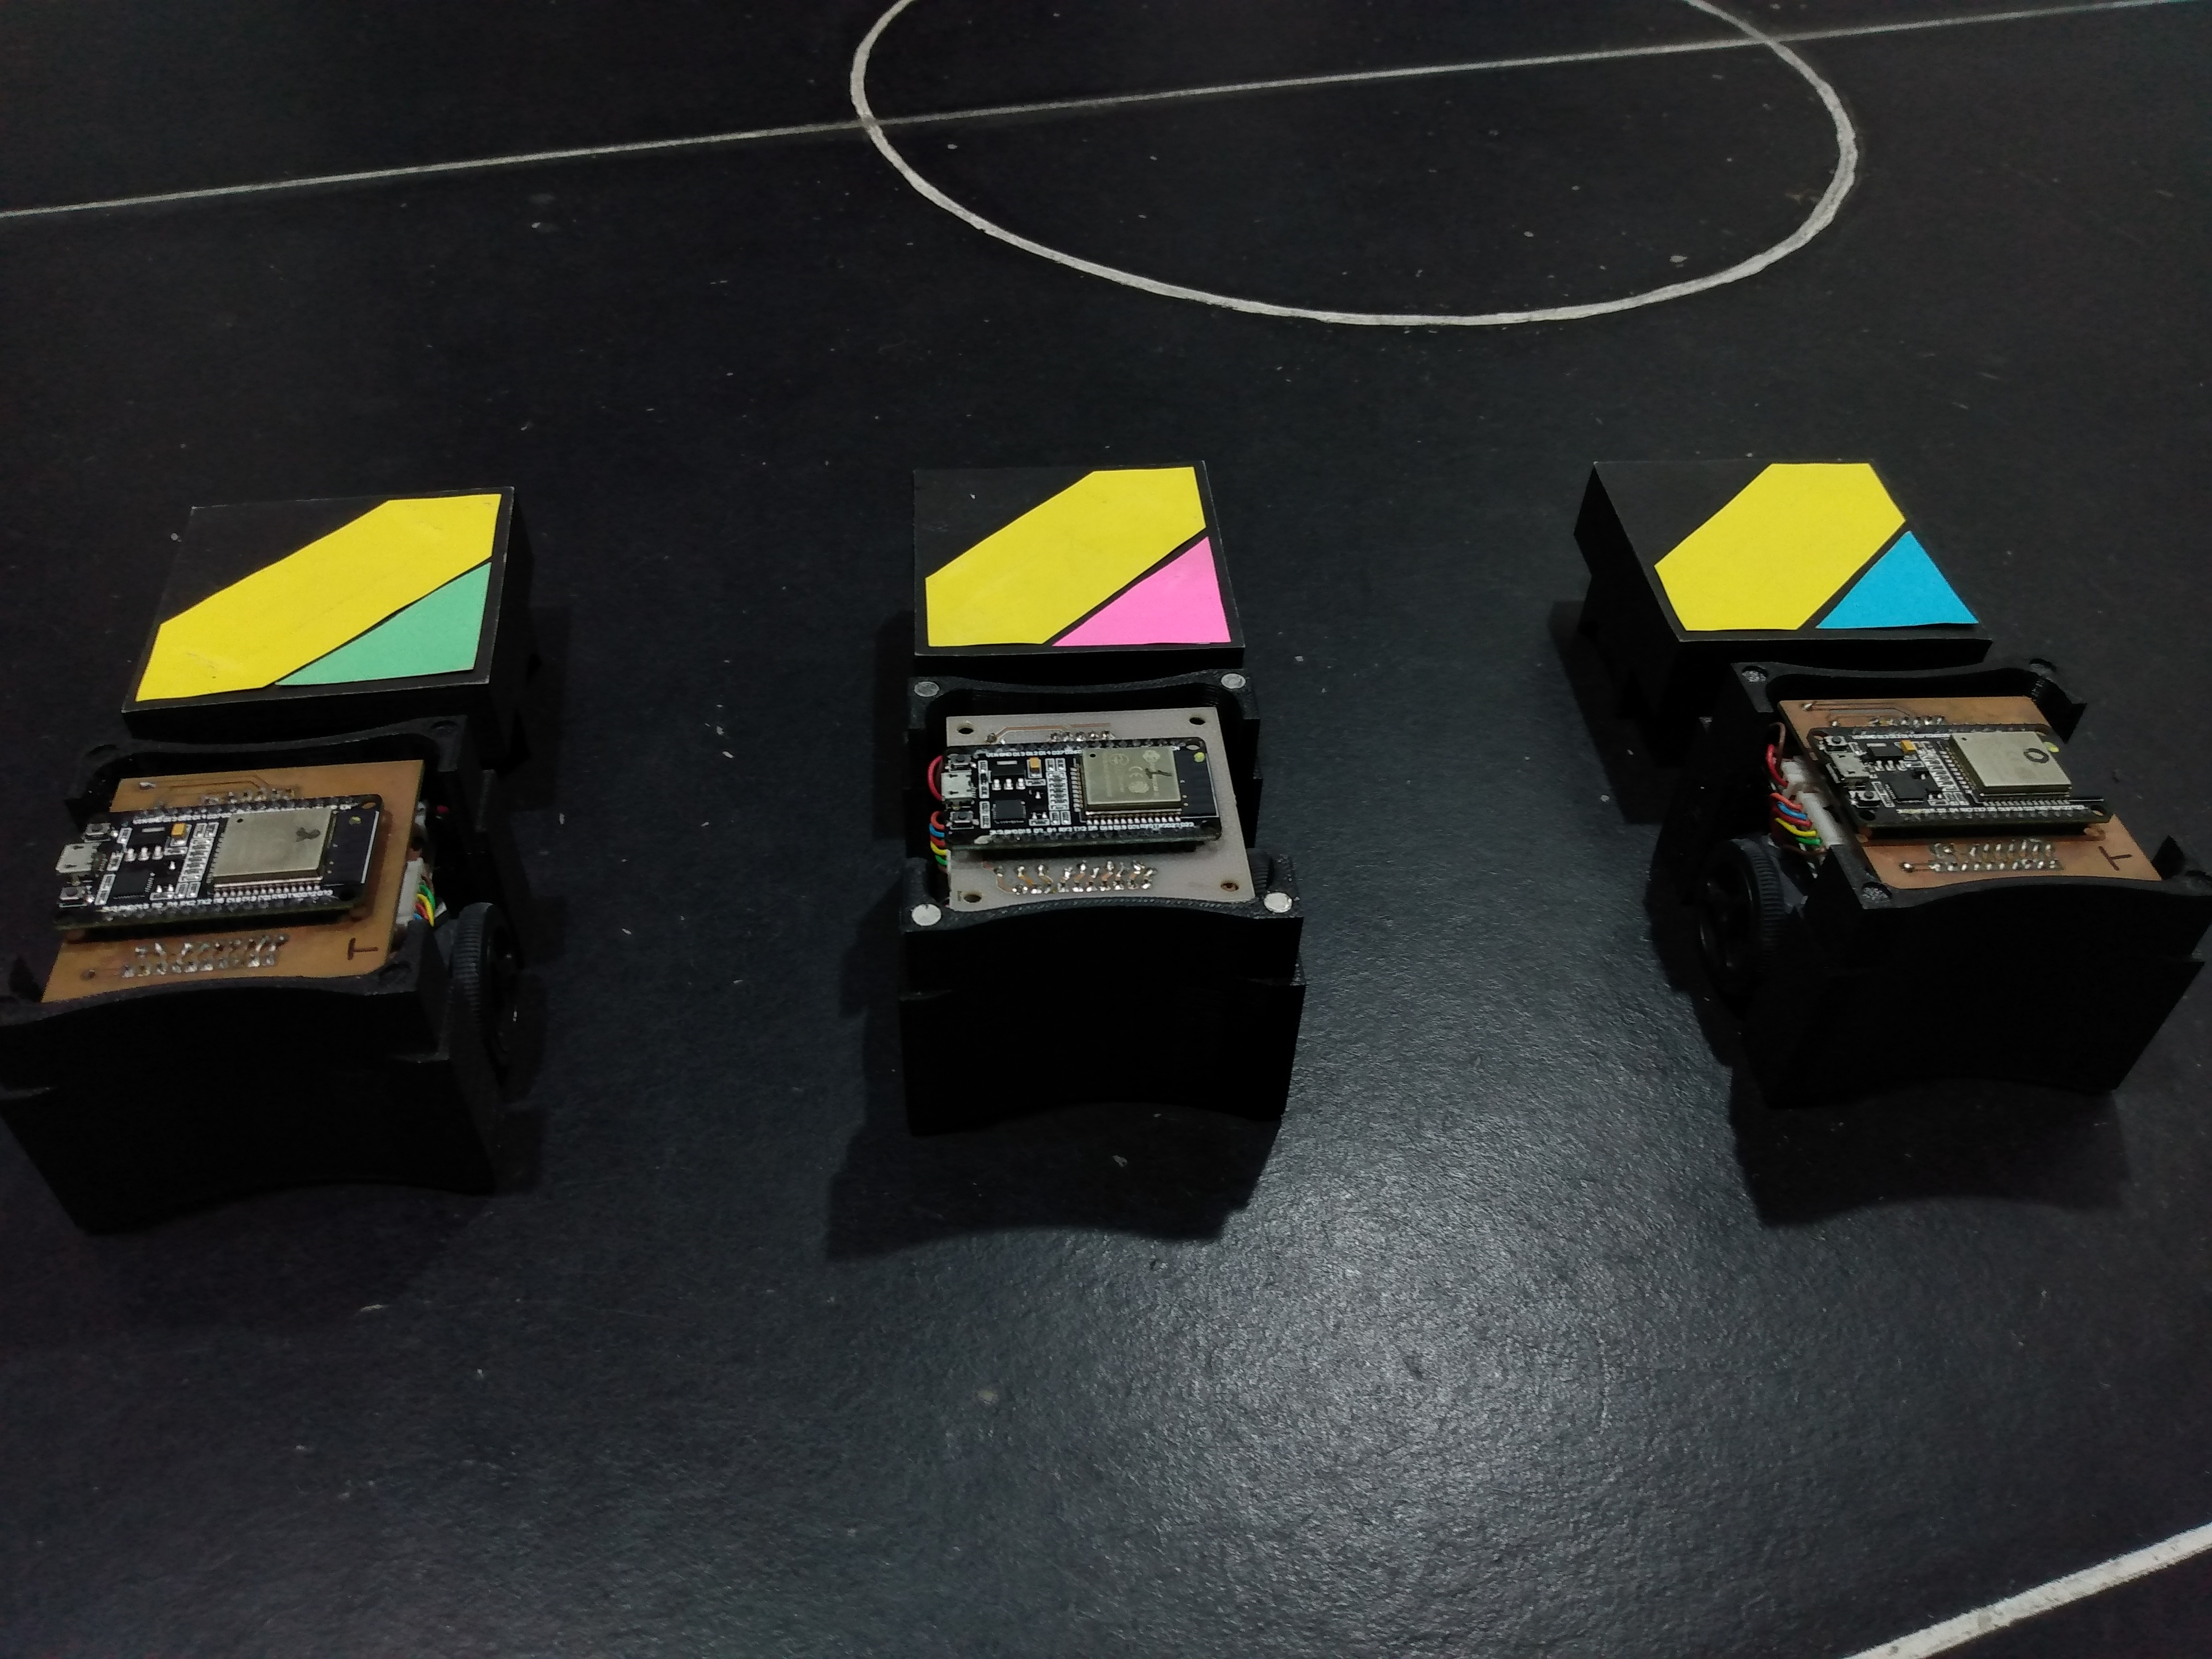
\includegraphics[width=0.4\textwidth]{figuras/robos/robos_capa_aberta.jpg}
        \caption{Robôs da Equipe POTI.}
    \end{figure}
\end{frame}


\begin{frame}{Projeto do Robô}
    \begin{figure}
        \centering
        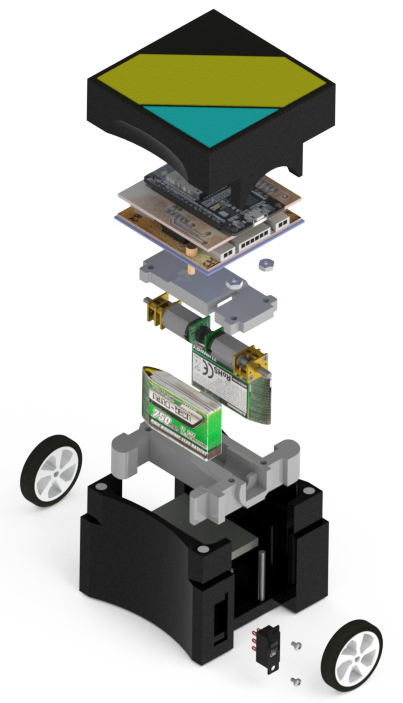
\includegraphics[width=0.3\textwidth]{figuras/robos/robo_completo_explodido.png}
        \caption{Visão geral do projeto dos robôs utilizados.}
    \end{figure}
\end{frame}

\begin{frame}{O Microcontrolador}

\begin{itemize}
    \item CPUs: 2 núcleos principais e um terceiro núcleo de baixo consumo enérgico. 
    \item Frequência de operação dos núcleos: Até $240$ MHz
    \item Interface \emph{Wireless}: Wi-Fi e Bluetooth (802.11 b/g/n/e/i);
    \item Memória: 448 Kb de ROM, 520 Kb de SRAM e 4 Mb de Flash.
\end{itemize}

\begin{figure}[H]
    \centering
    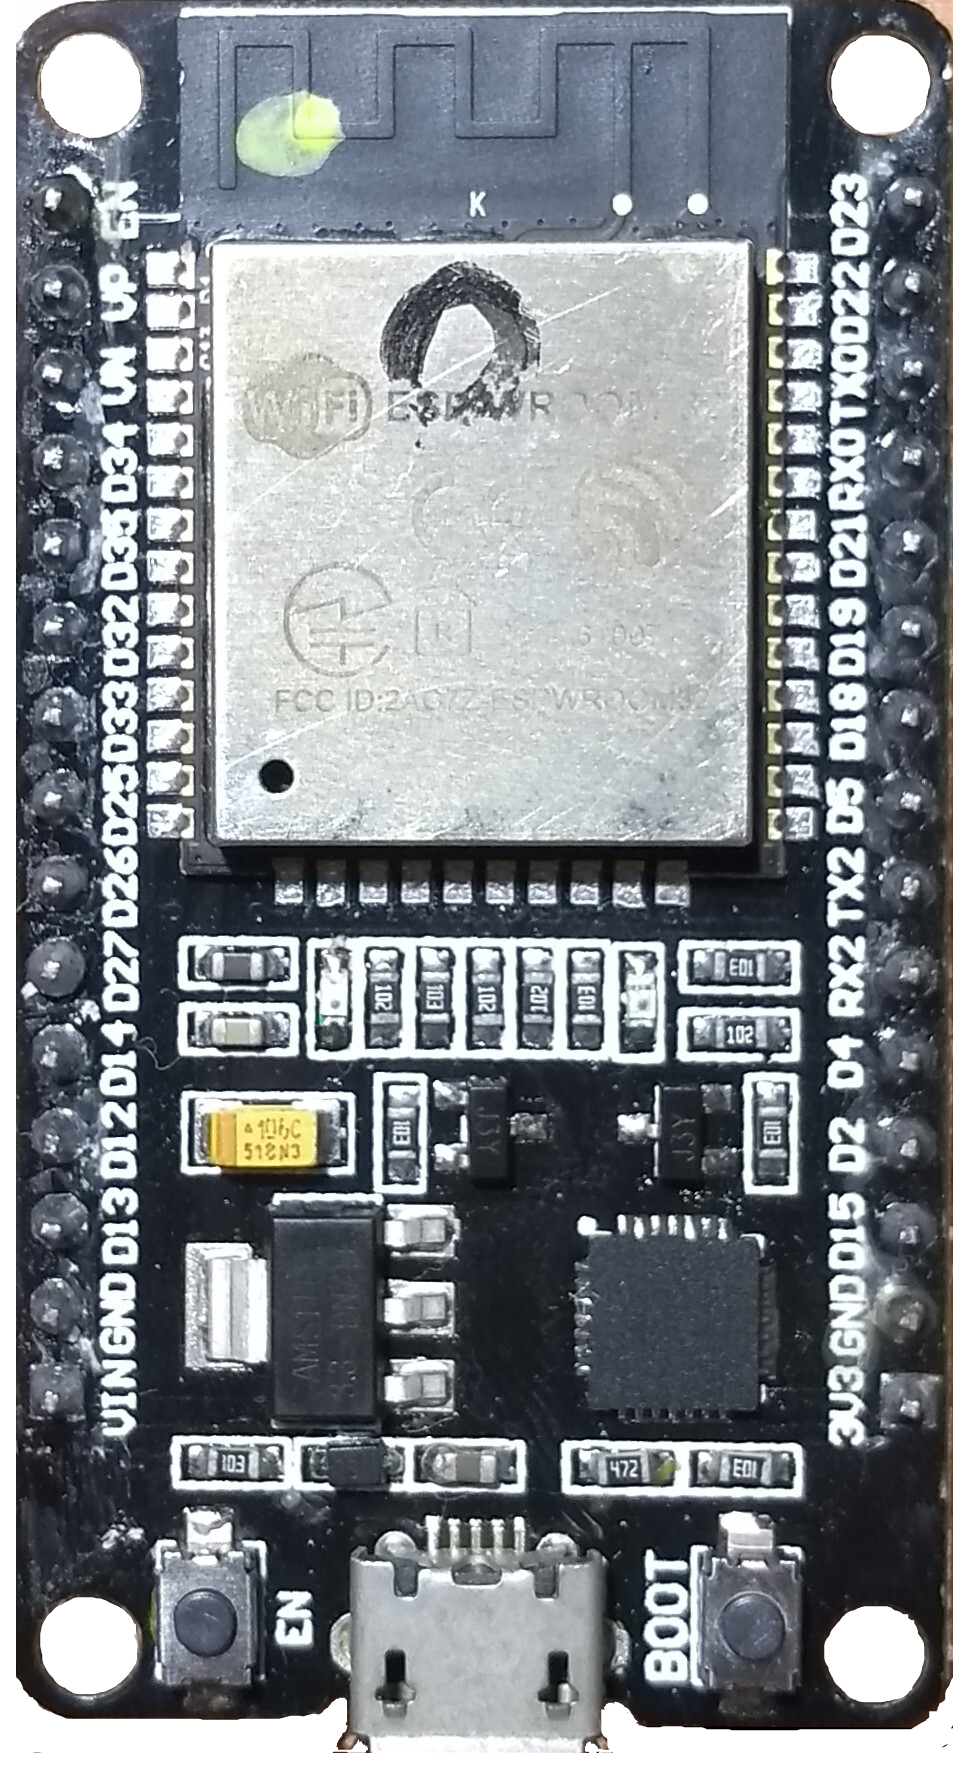
\includegraphics[width=0.1\textwidth]{figuras/eletronica/esp32_kit.png}
    \caption{Placa de desenvolvimento ESP32 Dev1.}
\end{figure}

\end{frame}

\begin{frame}{Conjunto Motor-Sensor}
    \begin{figure}
        \centering
        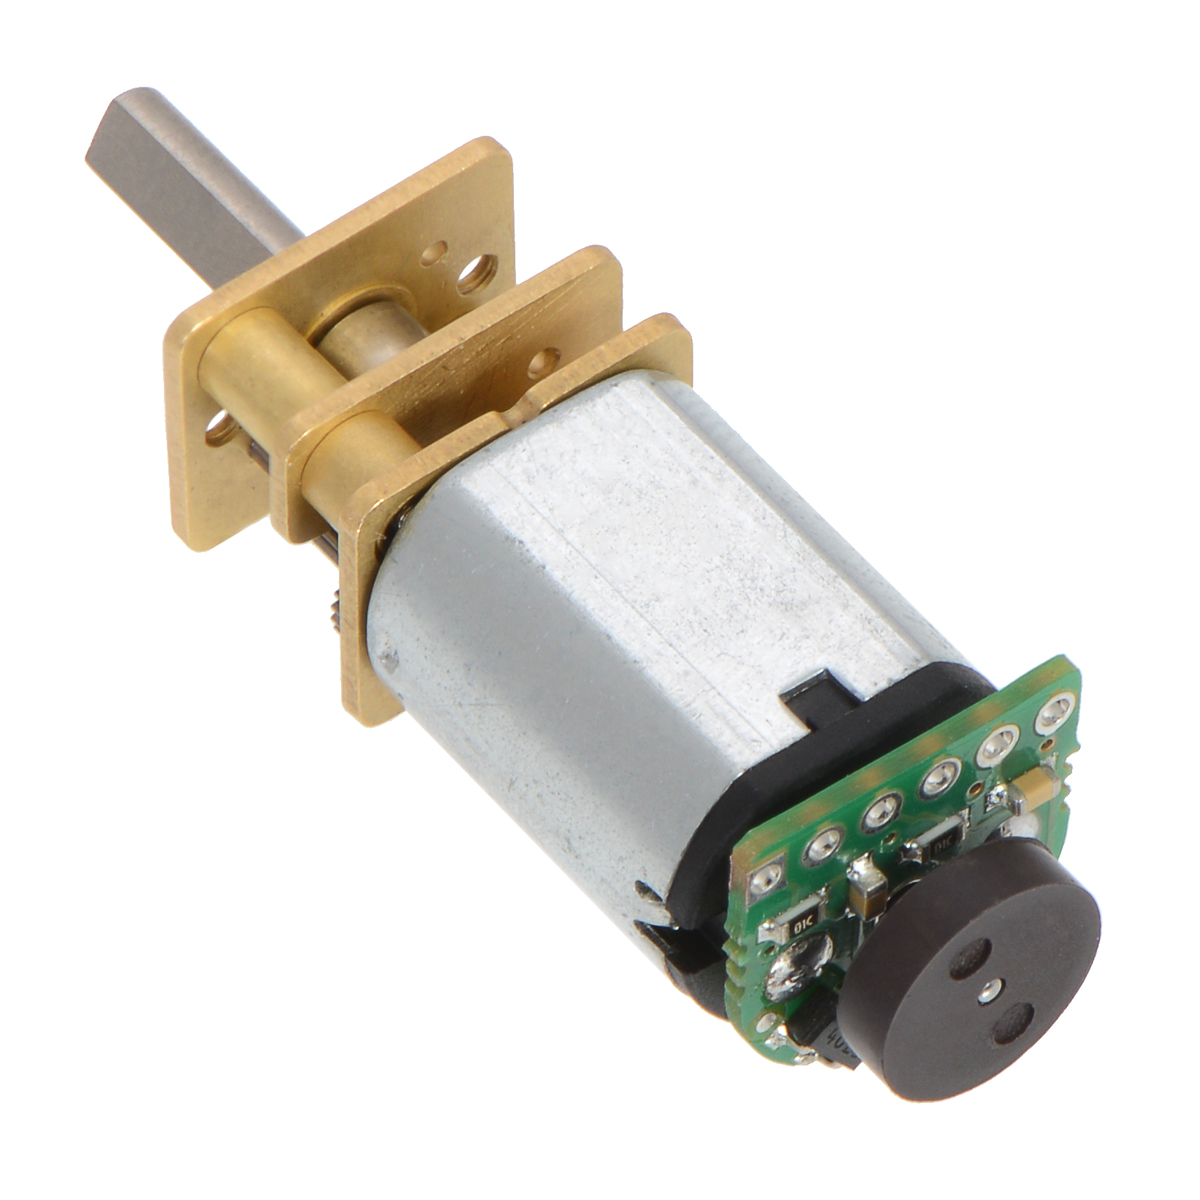
\includegraphics[width=0.4\textwidth]{figuras/eletronica/motor_com_encoder.jpg}
        \caption{Motor equipado com \emph{Encoder} magnético e caixa de redução de 30:1.}
    \end{figure}
\end{frame}

\subsection{\emph{Firmware}}

\begin{frame}{Divisão de Tarefas no $\mu{}C$}
    \begin{figure}
        \centering
        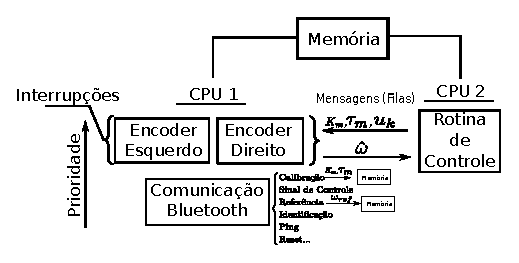
\includegraphics[width=1.0\textwidth]{figuras/ilustracoes/visao_geral_do_sistema.eps}
        \caption{Visão geral do sistema embarcado.}
    \end{figure}
\end{frame}

\begin{frame}{Rotina de Comunicação}
    
    \begin{figure}
        \centering
        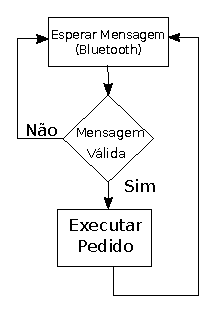
\includegraphics[width=0.5\textwidth]{figuras/ilustracoes/ilustracao_rotina_de_comunicacao.eps}
        \caption{Fluxo grama simplificado da rotina de comunicação.}
    \end{figure}
        
\end{frame}

\begin{frame}{Pacote de Mensagem}
    \begin{figure}
        \centering
        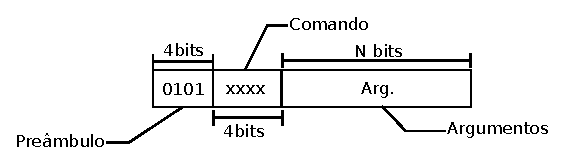
\includegraphics[width=1.0\textwidth]{figuras/ilustracoes/ilustracao_frame_generico.eps}
        \caption{Ilustração de um pacote genérico.}
    \end{figure}
\end{frame}

\begin{frame}{Comandos}
    \begin{align*}
    \text{Comandos}
        \begin{cases}
            \text{Pedir dados da Calibração:} & 0000\\
            \text{Realizar Calibração:} & 0100\\
            \text{Velocidades de Referência:} & 1010\\
            \text{Sinal de Controle:} & 1011\\
            \text{Velocidades Atuais:} & 0011\\
            \text{Iniciar rotina de coleta de dados(\emph{Identify}):} & 0101\\
            \text{Teste de conexão (\emph{Ping}):} & 1111
        \end{cases}
    \end{align*}
\end{frame}

\begin{frame}{Comando:Referência}
    \begin{figure}
        \centering
        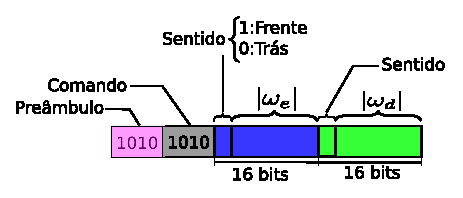
\includegraphics[width=\textwidth]{figuras/ilustracoes/ilustracao_comando_omega_ref.eps}
        \caption{Telecomando de velocidades de referência.}
    \end{figure}
\end{frame}

\begin{frame}{Comando:Sinal de Controle}
    \begin{figure}
        \centering
        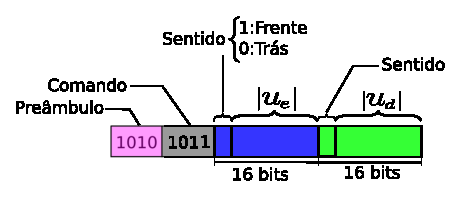
\includegraphics[width=\textwidth]{figuras/ilustracoes/ilustracao_comando_sinal_de_controle.eps}
        \caption{Telecomando de sinal de controle.}
    \end{figure}
\end{frame}

\begin{frame}{Comando:Coleta de Dados}
    \begin{figure}
        \centering
        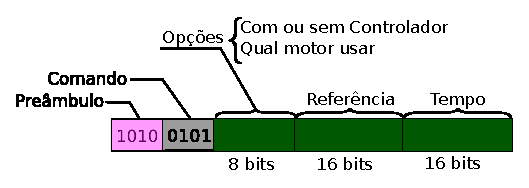
\includegraphics[width=\textwidth]{figuras/ilustracoes/ilustracao_comando_coleta_de_dados.eps}
        \caption{Telecomando para coleta de dados.}
    \end{figure}
\end{frame}

\begin{frame}{Rotina de Calibração}
    
\end{frame}

\begin{frame}{Rotina de Leitura dos Sensores}
    
\end{frame}

\begin{frame}{Rotina de Controle}
    
\end{frame}

\subsection{Experimentos e Validação}
\begin{frame}{Experimentos e Validação}
    
\end{frame}

